% Copyright 2007 by Till Tantau
%
% This file may be distributed and/or modified
%
% 1. under the LaTeX Project Public License and/or
% 2. under the GNU Public License.
%
% See the file doc/licenses/LICENSE for more details.
\documentclass{beamer}
\setbeamertemplate{bibliography item}[text]
\title{\textbf{Software Platform for Volunteered Computing using P2P}\\ \vspace{2.5mm} {\normalsize CS4089 Project\\Midterm Evaluation}}
\author{K C Sreevasthavan, Giridhar G Nair, Irfan T Naushad\\Guided By: Dr. Priya Chandran}
\date{March 17, 2016}
\usepackage{graphicx}

\begin{document}

\begin{frame}
  \titlepage
\end{frame}

\begin{frame}{Outline}
  \tableofcontents
\end{frame}
\section{Introduction}
\begin{frame}{Introduction}
\begin{itemize}
\item In this semester we have begun the implementation of our platform.
In this presentation we will be giving an overview of the work done till now, 
and also what we hope to complete by the final evaluation.
\end{itemize}
 
\end{frame}
\section{Problem Statement}
\begin{frame}{Problem Statement}
\begin{itemize}
\item To implement a software platform for
computing that uses P2P for communication / data-sharing between volunteering nodes.
\end{itemize}
\end{frame}

\section{Literature Survey }
\begin{frame}{Literature Survey}
Various P2P frameworks were considered such as Kurin's Py-P2P\cite{kurin}, Sameul Chen's\cite{chen} 
and Twisted Networking Engine\cite{twisted}. Official python documentation \cite{python} is being used as 
reference for development.
\end{frame}

\section{Work Done}
\begin{frame}{Work Done}
\begin{itemize}
\item The design of the platform we arrived in the previous semester.
\end{itemize}
\vspace{2ex}
\begin{center}
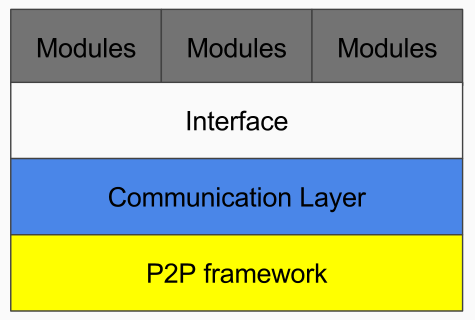
\includegraphics[scale=0.35]{pic3}
\end{center}
\end{frame}

%\begin{frame}{}
%\begin{itemize}
%\item Basic operation
%\end{itemize}
%\vspace{5ex}
%\includegraphics[scale=0.4]{proposed}
%\end{frame}

\begin{frame}{}
\begin{itemize}
\item Intercommunication between the nodes.
\begin{center}
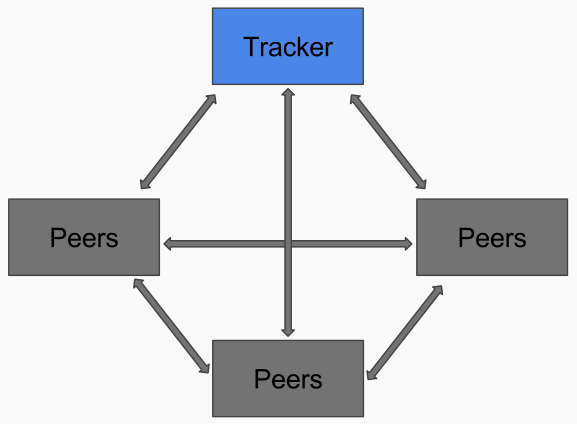
\includegraphics[scale=0.35]{pic}
\end{center}
\end{itemize}
\end{frame}

%\section{Work Done}
\begin{frame}{}
\begin{itemize}
\item We have revised the design of the platform.
\end{itemize}
\begin{center}
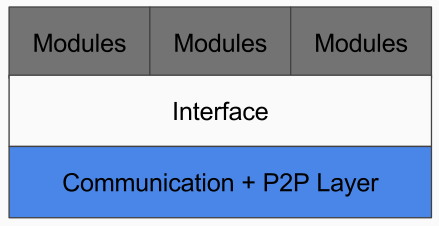
\includegraphics[scale=0.35]{pic2}
\end{center}
\begin{itemize}
\item Integrated Communication and P2P layer into one single layer
\end{itemize}
\begin{itemize}
\item Tracker nearly finalised. Handles Peerlist and modulelist
 manipulations, Account creation and login.
\end{itemize}
\end{frame}

\begin{frame}{}
\begin{center}
\begin{itemize}
\item Message format finalised.
\end{itemize}
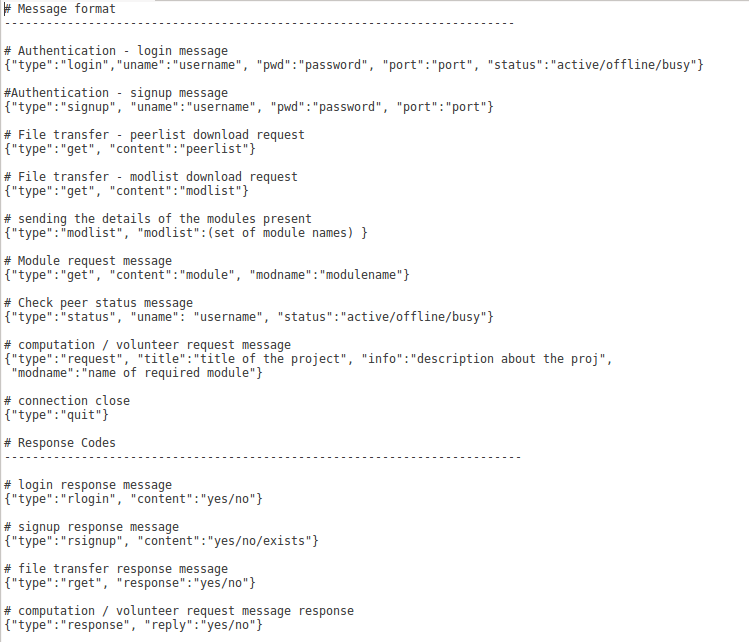
\includegraphics[scale=0.35]{msg}
\end{center}
\end{frame}

\section{Future Work}
\begin{frame}{Future Work}
\begin{itemize}
\item Completion of networking layer (communication + P2P layer) of the platform 
\end{itemize}
\begin{itemize}
\item Implementation of Interface layer
\end{itemize}
\end{frame}


\section{References}
\begin{frame}[allowframebreaks]
  \frametitle<presentation>{References}   
\begin{thebibliography}{}
\bibliographystyle{ieeetr}
\bibitem{kurin}
Kurin's Py-P2P \url{https://github.com/kurin/py-p2p}, Toby Burress.
\bibitem{chen}
P2Python \url{https://github.com/samuelchen/P2Python}, Samuel Chen.
\bibitem{twisted}
Twisted Event Driven Networking Engine \url{https://twistedmatrix.com/trac/}, Twisted Matrix Labs.
\bibitem{python}
Python 3.5.1 Tutorial \url{https://docs.python.org/3/tutorial/} Python Software Foundation.
\end{thebibliography}{}
%\bibliographys{group5}
\bibliographystyle{ieeetr}
\end{frame}

\end{document}

